\subsection{基于注意力机制的模型}\label{attention}
交互层是整个网络模型中关键的一层,前面的编码层输出的是问题和文章中每个单词的上下文语义编码,每个单词
关注了自己所在句子的上下文单词,但是却并没有关注对应的句子。而我们在做阅读理解问题时,通常是带着
问题去文章中找答案,我们要知道文章中每一个单词和问题之间的相关度。因此交互层的目的就是让文章的语义信息与问题的
语义信息融合,以此达到对文章更深层次的理解,而交互层中最常用的方法就是注意力机制。

注意力机制可以被视为是一个查询向量(query)和一组键值对向量(key-value pairs)的映射过程。整个过程首先是利用函数$f$衡量query和key之间的相似度,具体的就是生成一个权重分数向量,然后将权重分数向量归一化(通常利用softmax函数)后对value加权求和得到的结果就是query对key-value pairs的注意力。具体计算公式形式如下:

\begin{gather}
\alpha_i=\text{softmax}(f(Q,K_i)) \notag \\
\text{Attention}(Q,K,V)=\sum_{i=1}^{n}\alpha_iV_i
\end{gather}
其中$(K_i,V_i)$代表key-value pairs中的第$i$个值,
函数$f$常采用计算方式有内积函数、二次型函数、
单层前馈神经网络,双维度转换函数,分别见如下公式:
\begin{gather}
f(p_i,Q)=p_i^TQ \qquad \text{内积函数} \\
f(p_i,Q)=p_i^TWQ\\
f(p_i,Q)=v^T\tanh(Wp_i+UQ) \\
f(p_i,Q)=p_i^TW^TUQ 
\end{gather}

在NLP领域中$K=V$,简单的来说就是两个序列中其中一个序列为另一个序列的每一个位置生成一个权重值,这个值代表当前位置的单词对另一个序列的重要性。
如果是自注意力(self attention),那么此时$Q=K=V$,目的是计算序列中某个单词和其它单词之间的相关性从而增强自身的语义表示。
Bahdanau等人\upcite{Bahdanau}最早将
注意力机制应用在机器翻译领域,获得了极大的反响,
为NLP领域的其它任务的模型提供了启发式的思想。
以下将首先介绍MRC任务中注意力机制之间的差异,然后分析各个模型如何将注意力机制应用在MRC任务上以及它们之间的区别与联系。

\subsubsection{MRC中的注意力}
% 单方向注意力的运算机制类比于人类做阅读问题的过程: 带着问题到文章中找答案,从文章的角度
% 对问题进行总结,获得文章对问题的注意力。
% 也就是先看问题,然后对于文本段落中各个部分生成一个注意力权重,代表这个部分与问题的相关程度,
% 利用注意力权重对文本的各个部分加权求和就可以得到文本段落与问题之间的相关性信息。
MRC模型做注意力运算有两个方向,即从问题到文章,从文章到问题这两个方向。从问题到文章的注意力是指
将问题看做是$Q$,文章看做$K,V$。利用问题去和文章做注意力计算,得到问题对文章的注意力权值,它代表问题对文章每一个单词的关注程度,利用它对文章的语义表示向量加权求和得到的就是问题的一个新的语义表示。
从文章到问题注意力类似,此时文章看作是$Q$,问题看做$K,V$,利用文章和问题做注意力计算,即文章的每一个单词都会
关注到问题,然后利用注意力权值对问题加权求和从而计算得到文章的新的语义表示。
以问题到文章的注意力计算过程为例,$P=[p_1,p_2,\cdots,p_n] \in R^{n\times d},Q\in R^{d}$代表文章的语义信息,其中$n$代表文章长度,$d$代表向量维度,每一个
$p_i$代表文章中单词的语义向量表示,$Q$代表整个问题的语义信息。问题到文章的注意力计算步骤如下:
\begin{gather}
	\alpha_i=\text{softmax}(f(p_i,Q)) \notag \\
	\text{Attention}(P,Q)=\sum_{i=1}^{n}\alpha_{i}p_i \notag 
\end{gather}
%就是利用问题
%的语义信息和文章中每一个单词的向量表示计算它们之间的相关性,最后得到一组注意力权重$\alpha=[\alpha_1,\alpha_2,\cdots,\alpha_n]$
%表示文章与问题之间的相关程度,利用$\alpha$对文章加权求和就可以提取出来文章中与问题最相关的单词,
%这些单词对于回答问题是至关重要的。

上面的式子是将问题压缩成一个固定维度的向量,得到的注意力权重也是一维的,因此也成为一维注意力。
一维注意力方法所关注的是问题序列的整体对文章的注意力,没有考虑问题序列的不同单词之间对文章的关注程度差异。
与其相对应的是二维注意力,即对于问题序列中的
每一个单词都会和文章做注意力计算,得到的注意力权重是二维向量。

文章到问题注意力可以看做是带着文章阅读问题,问题到文章则可以看做是带着问题阅读文章。这两种都属于交互的计算注意力,然而这种注意力机制可能导致只重视文章中与问题相关度高的单词,而忽视了文章所强调自身的语义信息。在文章上利用自注意力机制则可以看做是反复的阅读文章,从而加深对文章语义信息的理解。

如果按照注意力的计算次数上区分,
又可以分为one-hop和multi-hop形式。one-hop,也叫“单跳结构”是指仅仅通过一次计算得到注意力权值然后加权求和得到注意力结果,这也是一种
静态的计算形式。与之对应的是multi-hop,也叫“多跳结构”。one-hop形式下仅仅只做一次交互计算,而注意力机制虽然可以提取相关的重要信息,但是
它仍然是基于浅层语义信息的相似度计算。在机器阅读理解任务中,
对于复杂的问题通常是不能在一个句子中找出答案,需要多步推理才能寻找答案,如图1中
的例子:
\begin{figure}[ht]
    \centering
    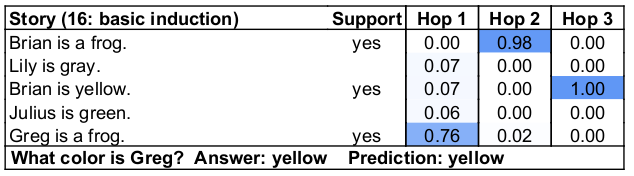
\includegraphics[width=0.5\textwidth]{end2end.png}
    \caption{MemN2N\upcite{MemN2N}提出的多步推理的一个样例 \\ Figure 1 An example of multi-hop reasoning from MemN2N}
\end{figure}
% \begin{figure*}
%     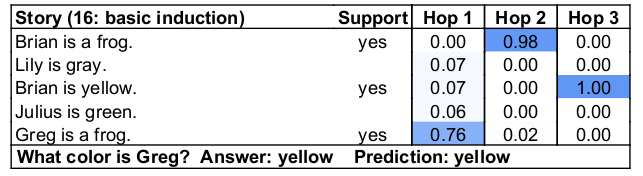
\includegraphics[]{multihop.png}
% \end{figure*}
%当前时刻计算的注意力结果要保留到下一时刻,即每一时刻都要计算注意力,是一种动态的计算形式,典型的代表是Bahdanau注意力\cite{neural machine translation by jointly learning to align and translate}。
我们可以看到想要得到最终的答案需要进行三次推理过程,在每一个推理过程中都会变换注意力关注的对象,显然one-hop结构是不能实现多步推理的。
实现多步推理这种机制通常有三种方式:
\begin{enumerate}
\item 基于之前时间步所计算得到的问题感知的文章语义信息计算下一时间步的文档和问题交互,如Impatient Reader\upcite{Hermann}。
\item 利用RNNs这种基于上一时刻隐藏状态更新下一时刻隐藏状态的循环特性来达到多步推理,如
Match-LSTM\upcite{MatchLSTM}。
\item 引入额外的记忆单元存储语义信息,目的是希望解决RNN中不能够长期依赖导致信息丢失的问题,典型
的如Weston等\upcite{MN}
提出的记忆网络(memory networks)。
\end{enumerate}

%上面的注意力计算都属于互注意力,即文章和问题两者之间做交互。此外还有自注意力机制(self-attention),自注意力机制是文本的向量表示和自身做交互,用来获得文本内部各个单词之间的依赖关系。

\subsubsection{相关模型}

%\subsubsection{Attentive Reader and Impatient Reader}
文献\cite{Hermann}最早利用神经网络模型并且融入注意力机制做MRC任务。
文中提出两种不同的单向注意力机制Attentive Reader
和Impatient Reader,均是计算问题到文章的注意力。
Attentive Reader是将问题表示为一个固定长度的向量然后与文章中每一个单词做注意力计算,然后利用注意力权重对文章
中的单词的向量表示加权求和得到一个固定长度的
向量即为注意力运算后的结果,然后与问题联合预测答案,其中注意力的运算方式采用加法模型(公式4)。可见这种注意力的计算方式仅仅只计算一次,因此属于one-hop类型。
Impatient Reader计算注意力的机制属于一种multi-hop的计算。并不是将
问题表示为一个固定长度的向量,而是对于问题中的每一个单词都要和整个文章做注意力计算,而且计算的结果
要和下一个单词以及文章共同做注意力计算,最后一个单词的注意力结果作为整个Impatient Reader计算注意力过程的结果。
这种方式类似于人在阅读过程中不断的在问题和文章之间做关注。
文献\cite{AR}在Attentive Reader的基础上利用双线性项(公式3)取代原有的利用tanh函数的加法模型(公式4)并且直接将
对文章加权求和后得到的向量作为预测答案的输入而不是联合问题$Q$的语义信息,实验证明这种简化反而提高了模型的准确度。

文献\cite{IAReader}提出Iterative Attention Reader(IA Reader)模型,利用BiGRU存储每一次
迭代计算得到的问题和文章的交互信息。在每一时间步上,首先利用上一次的BiGRU的状态与问题做一维注意力匹配提取出问题的语义信息,
然后再结合上一次的BiGRU的状态与文章再做一维注意力匹配从而提取出文章的语义信息。将问题与文章的语义信息
通过各自的门控单元作为BiGRU当前时刻的输入,其中门控单元采用前馈神经网络用来解决当前时间步下问题和文章的语义信息提取不充分的问题。
文献\cite{GAReader}提出Gated Attention Reader(GA Reader)模型,类似于IA Reader模型,同样采用
BiGRU作为编码模块实现多跳结构。在每一步的推理过程中,首先通过BiGRU得到问题的语义信息然后对文章的
每一个单词做注意力的计算得到问题感知的文章表示,同时采用点乘计算的门控机制建模问题感知的文章表示和原来的文章语义向量之间的交互关系,目的是利用问题更新文章的语义表示。这种处理过程
类比于带着问题反复的阅读文章,每一次都加深对文章的语义理解。

%基于注意力机制的模型大部分是利用RNN的循环机制来存储每次交互的状态,
%但是由于RNN的梯度消失问题可能会丢失语义信息,因此文献\cite{memory network}提出一种记忆网络架构(memory network),
%通过外部记忆模块来存储语义信息,但是这种记忆网络并不能端到端的训练。
%为了处理这个问题,文献\cite{MemN2N}提出一种端到端的记忆网络(MemN2N)。
%利用记忆槽存储文档中每一个句子的嵌入矩阵,记忆槽的状态以及问题的语义信息会随着与文档的多次交互不断更新。

文献\cite{Reasonet}提出一种动态决定推理次数的模型ReasoNet,不像之前的模型如GA Reader
,IA Reader等在整个推理过程中有着固定的推理次数。这种固定推理次数的缺点就是不考虑问题的复杂性,
对于复杂的问题往往需要模型多次的推理,因此不同题目难度需要不同的推理次数,应当让模型学会什么时候终止推理。为了达到这一目的,
ReasoNet模型利用一个终止门产生二元值输出来动态的决定是否继续推理。Reasonet模型大致分为外部记忆单元模块、内部控制器模块、终止门模块以及答案输出模块。
具体的,将文章和问题通过Bi-GRU编码后的语义表示作为
外部的记忆单元$M$,利用内部控制器(采用GRU)当前时刻的状态与$M$做二维注意力匹配,得到注意力结果输入到内部控制器中
更新内部控制器的状态。终止门模块以当前时刻内部注意力的状态作为输入来判断是否需要继续推理。由于产生了二元离散输出值,
使得模型不能用梯度下降法训练,因此模型引入强化学习机制训练。

%\subsubsection{Match-LSTM}
文献\cite{MatchLSTM}提出一种Match-LSTM网络,利用RNNs的循环机制达到多跳结构。
与之前模型如Impatient Reader不同,
虽然Match-LSTM也是多跳结构,并且也是一维注意力,但是
Match-LSTM计算的方向是文章到问题的注意力,将问题的语义信息融入到Match-LSTM中。
计算方式采用加法模型。具体计算过程如下:
\begin{gather}
    s_t=v^T\tanh(W^QH^Q+W^Ph_t^P+W_rh_{t-1}^r) \notag \\
    \alpha_{t}=\text{softmax}(s_t)
    %c_t=\sum_{i=1}^{m}a_i^tu_i^Q
\end{gather}
其中$H^Q$是问题通过编码层的输出,$h_t^P$是文章的第$t$个单词通过编码层的输出,$h_{t-1}^r$是Match-LSTM上一时刻
的隐藏状态。
$\alpha_{t}$是
文章的第$t$个单词与问题的每一个单词之间的注意力权重。
计算得到的注意力权重对问题的语义表示加权求和,此时得到的是关注问题的向量表示,然后与文章当前时刻单词的上下文表示拼接作为
Match-LSTM当前时刻的输入。
\begin{gather}
    z_t=[h_t^p;\alpha_tH^q] \notag \\
    h_{t}^r=\text{LSTM}(z_t,h_{t-1}^r)
\end{gather}
此外为了使得文章从后向前的对问题做关注,模型将文章序列翻转再次按照上述方式计算,最后将两个方向的计算结果
拼接作为交互层的输出。

文献\cite{RNet}提出一种带有门控机制的注意力循环神经网络以及自注意力机制联合的交互层设计模型,
也叫RNet。RNet在交互层的设计分为两部分。
第一部分是带有门控机制的注意力循环神经网络,整体计算
方式类似于Match-LSTM,而且额外加入了门控机制使得模型可以有选择的输出
语义信息。具体的,在公式(6)中的$z_t$上添加一个门控单元:
\begin{gather}
g_t=\text{sigmoid}(W_gz_t)\notag \\
z_t^{*}=g_t\odot z_t
\end{gather}
其中$\odot$表示元素之间的点乘。
由于$z_t=[h_t^p;\alpha_tH^q]$,$h_t^p$表示的是文章的第$t$个单词的语义表示,$\alpha_tH^q$表示的是
对问题语义表示的融合,因此
通过添加门控单元使得模型可以有选择的决定哪部分作为重要的语义信息输出。这种机制类似于人在阅读过程中要
忽略文章中那些与问题无关的信息,凸显出重要的信息才能更加准确的找到答案。
第二部分是利用自注意机制对文章的语义信息再次交互建模。基于注意力机制的循环神经网络的输出对关注了问题的
文章语义表示与原始文章语义表示建模后的输出,而这种计算机制的问题之一是
两个距离较远的单词之间交互信息由于梯度消失等原因会变得很弱。因此
通过自注意机制可以使得文章中每一个单词关注到其余所有的单词,使得模型对文章达到更深层次的理解。

% 文献\cite{FusionNet}提出一种融合网络(FusionNet),所谓融合就是指将问题与文章的语义信息交互,然后将文章的语义信息融合到问题中以及将
% 问题的语义信息融合到文章中,一个好的融合机制很大程度上影响模型的性能。一般认为对于网络中较低的层所表达的是语法层面的特征,
%下表详细的对比了本文介绍的所有基于注意力机制的模型之间的差异。

%\begin{table}
%	%\text{基于注意力机制的模型对比}
%	\centering
%	\caption{基于注意力机制的模型对比}
%	\vspace{10pt}
%	%\resizebox{\linewidth}{!}{
%	\begin{tabular}{c c c c}
%		\toprule
%		模型&注意力方向&注意力维度&推理模式 \\
%		\midrule
%		Attentive Reader\upcite{Hermann}&Q2C&one-dim&one-hop \\
%		\midrule
%		Impatient Reader\upcite{Hermann}&Q2C&two-dim&multi-hop \\
%		\midrule
%		Standford Reader\upcite{AR}&Q2C&one-dim&one-hop \\
%		\midrule
%		AS Reader\upcite{ASR}&Q2C&one-dim&one-hop \\
%		\midrule
%		IA Reader\upcite{IAReader}&Q2C&one-dim&multi-hop \\
%		\midrule
%		GA Reader\upcite{GAReader}&C2Q&two-dim&multi-hop \\
%		\midrule
%		Match-LSTM\upcite{MatchLSTM}&C2Q&two-dim&multi-hop \\
%		\midrule
%		DCN\upcite{DCN}&\tabincell{c}{C2Q \\
%			Q2C}&two-dim&one-hop \\           
%		\midrule
%		BiDAF\upcite{BiDAF}&\tabincell{c}{C2Q\\ Q2C}&two-dim&one-hop \\
%		\midrule
%		ReasoNet\upcite{Reasonet}&\tabincell{c}{C2Q\\ Q2C}&two-dim&multi-hop\\
%		\midrule
%		R-Net\upcite{RNet}&C2Q&two-dim&multi-hop \\
%		\midrule
%		QANet\upcite{QANet}&\tabincell{c}{C2Q\\ Q2C}&two-dim&one-hop\\
%		\bottomrule
%	\end{tabular}
%	%}
%\end{table}
之前的模型在交互层利用注意力机制融合文章和问题时,无论是单向还是双向注意力,它们都是利用句子的高层级别的语义信息即编码层的输出,而忽略了句子在低层次级别的语义信息如单词级别的词嵌入等。文献\cite{Fusionnet}提出FusionNet模型,目的就是保留多个层次的语义信息,即将每一个单词在第一层到后面所有层的向量表示拼接成一个向量,原文中称为单词历史(history of word),因为它包含了一个单词所有层的语义编码。但是随着层数的增加维度会变得越来越大,为了解决维度问题同时不损失单词的历史信息,FusionNet提出全关注注意力机制的概念:即利用文章和问题的单词历史计算得到注意力权重,然后对问题的某一层语义向量加权求和。这种机制使得两个输入向量可以互相关注到对方的历史信息同时压缩维度。此外文中对注意力权重的计算方式如下:
\begin{equation}
\alpha_i=\text{ReLU}(Up_i)^TD\text{ReLU}(Uq_j)
\end{equation}
其中$p_i\in R^d$和$q_j\in R^d$分别代表文章第$i$个单词和问题第$j$个单词的单词历史,$U$和$D$是训练的参数。


%Match-LSTM仅仅计算文章到问题的注意力,并未考虑问题到文章的注意力。

%\subsubsection{DCN}
上述的模型全都属于单方向注意力,要么仅计算文章到问题的注意力或者仅计算问题到文章的注意力。
文献\cite{DCN}提出一种Dynamic Co-attention Network(DCN)模型,
在交互层中采用协同注意力机制,
协同注意力同步的计算文章对问题的注意力以及问题对文章的注意力。
最后按照公式(9)融合两个两个方向的注意力作为交互层的输出。
\begin{equation}
\widetilde{C}=\beta[Q,\alpha C]
\end{equation}
其中$\alpha$和$\beta$分别表示文章与问题之间的注意力权重,$\widetilde{C}$同时融合了问题的语义信息和文章的语义信息。
文献\cite{BiDAF}提出(Bidirectionl Attention Flow,BiDAF)模型。
同样计算两个方向(C2Q和Q2C)的注意力,但是与之前模型不同的是BiDAF将之前的文章语义表示和交互层计算得到的问题感知的文章语义表示一起流向后面的层,这样一定程度上避免了过早的对文章语义信息概括而导致
信息的损失。模型的简化实验表明C2Q方向的注意力对模型的重要性大于Q2C方向的注意力,一种可能的原因是由于问题序列的长度小于文章的长度所以计算得到的文章感知的问题语义向量的信息不够充分。
%BiDAF的计算方式如下:
%\begin{gather}
%    S=W^T[C;Q;C\circ Q]\in R^{m\times n} \notag \\
%    \widehat{Q}=\text{softmax}(S)Q \in R^{m\times d}\notag \\
%    \alpha=\text{softmax}(\max_{col}(S)) \in R^{m}\notag \\
%    \widehat{c}=\sum_{i=1}^{m}\alpha_tC_{:i}\in R^{d}
%\end{gather}
%其中$C,Q$分别表示文章和问题的语义向量表示,$m,n$分别表示文章和问题的长度,
%$S$表示文章和问题之间的相似度矩阵,$\circ$表示点乘运算。$\widehat{Q}$表示的就是文
%章对问题的注意力,即代表着问题中哪个单词与文章最相关。
%$\alpha$的意义是将关于问题最相关的文章中的单词提取出来,这些单词是作为答案的关键因素。
%$\widehat{c}$就是将文章
%中与问题最相关的单词的语义向量加权求和,将其重复$m$次得到问题对文章的注意力$\widehat{C}$。
%最后以如下形式作为BiDAF交互层的输出:
%\begin{gather}
%    [C;\widehat{Q};C\circ \widehat{Q};C\circ \widehat{C}]
%\end{gather}
%此外实验结果表明去掉文章到问题的注意力后模型效果显著下降。

%\subsubsection{RNet}




%\subsubsection{QANet}
文献\cite{QANet}提出一种网络模型QANet,不像之前的那些模型几乎都是用RNNs来做编码器,
QANet提出一种新颖的编码结构,利用卷积结合transformer\upcite{Transformer}中的
多头注意力结构
。
卷积方式采用的是文献\cite{DSC}提出的深度可分离卷积(depthwise 
separable convolutions),
相比传统的卷积计算方式深度可分离卷积可以减少运算次数。
整个结构的思想是先利用卷积操作建模局部特征的交互,再用自注意力机制建模全局交互,
实验结果表明这种架构不仅加快训练速度同时在SQuAD数据集上模型性能优于那些利用RNNs作为编码器的模型。
%QANet交互层的计算方式借鉴于BiDAF和DCN两个模型的计算方式。

表6详细的对比了本文介绍的所有基于注意力机制的模型之间的差异。其中Q2C代表问题到文章注意力,C2Q代表文章到问题注意力,one-dim代表一维注意力,two-dim代表二维注意力,one-hop代表单跳结构,multi-hop代表多跳结构。
\begin{table}[ht]
	%\text{基于注意力机制的模型对比}
	\centering
	\caption{基于注意力机制的模型对比 \\ Table 6 Comparison of models based on attention mechanism}
	%\vspace{10pt}
	%\resizebox{\linewidth}{!}{
	\begin{tabular}{c c c c}
		\toprule
		模型&注意力方向&注意力维度&推理模式 \\
		\midrule
		Attentive Reader\upcite{Hermann}&Q2C&one-dim&one-hop \\
		\midrule
		Impatient Reader\upcite{Hermann}&Q2C&two-dim&multi-hop \\
		\midrule
		Standford Reader\upcite{AR}&Q2C&one-dim&one-hop \\
		\midrule
		AS Reader\upcite{ASR}&Q2C&one-dim&one-hop \\
		\midrule
		IA Reader\upcite{IAReader}&Q2C&one-dim&multi-hop \\
		\midrule
		GA Reader\upcite{GAReader}&C2Q&two-dim&multi-hop \\
		\midrule
		Match-LSTM\upcite{MatchLSTM}&C2Q&two-dim&multi-hop \\
		\midrule
		DCN\upcite{DCN}&\tabincell{c}{C2Q \\
			Q2C}&two-dim&one-hop \\           
		\midrule
		BiDAF\upcite{BiDAF}&\tabincell{c}{C2Q\\ Q2C}&two-dim&one-hop \\
		\midrule
		ReasoNet\upcite{Reasonet}&\tabincell{c}{C2Q\\ Q2C}&two-dim&multi-hop\\
		\midrule
		R-Net\upcite{RNet}&C2Q&two-dim&multi-hop \\
		\midrule
		QANet\upcite{QANet}&\tabincell{c}{C2Q\\ Q2C}&two-dim&one-hop\\
		\bottomrule
	\end{tabular}
	%}
\end{table}

%One possible interaction for the operation C^QA^D is tha mapping of question encodings into space
%of passage encodings

% \begin{table*}[ht]
%     \centering
%     \caption{模型对比}
%     \vspace{10pt}
%     \begin{tabular}{l c c c}
%         \toprule
%         \multirow{2}{*}{模型}&SQuAD 1.1\upcite{SQuAD1}& SQuAD 2.0\upcite{SQuAD2} & RACE\upcite{RACE}\\
%         \cmidrule(lr){2-2} \cmidrule(lr){3-3} \cmidrule(lr){4-4}
%         &EM/F1&EM/F1& acc \\
%         \midrule
%         Match-LSTM\upcite{MatchLSTM}& 64.7/73.7 & -&-\\
%         \midrule
%         DCN\upcite{Dynamic coattention networks for question answering}& 66.2/75.9 &-&-\\
%         \midrule
%         ReasoNet\upcite{Reasonet}&70.6/79.4 &-&-\\
%         \midrule
%         BiDAF\upcite{Bidirectional attention flow for machine comprehension}&68.0/77.3 &-&-\\
%         \midrule
%         R-Net\upcite{RNet}&72.3/80.7 &-&-\\
%         \midrule
%         QANet(data augmentation x3)\upcite{QANet}& 76.2/84.6&-&-\\
%         \midrule
%         ELMo+BiDAF\upcite{ELMo}&78.6/85.8&-&-\\
%         \midrule
%         GPT-v1\upcite{GPT}&-&-&59.0\\
%         \midrule
%         $\text{BERT}_{large}$(+TriviaQA)\upcite{BERT}& 85.1/91.8 &80.0/83.1&72.0\\
%         \midrule
%         XLNet\upcite{XLNet}&-&86.4/89.1 &81.8\\
%         \midrule
%         RoBERTa\upcite{RoBERTa}&-&86.8/89.8 &83.2\\
%         \midrule
%         ALBERT\upcite{ALBERT}&-&88.1/90.9 &86.5\\
%         \bottomrule
%     \end{tabular}
% \end{table*}










